\section{Data treatment}
\label{sec:DataTreatment}

Having the extracted neuropil corrected fluorescence traces, F, for all of the session's time, it is also required to extract $\Delta F/F$ traces: these indicate the measured changes in fluorescence between the cell's peak stimulation times and resting state and serve as the actual data measurements to use in all of subsequent analysis.

For every ROI's trace response, the baseline fluorescence ($F_0$) was estimated by discarding the tails of the fluorescence trace distribution and taking the mean fluorescence, using a 60 s sliding window. The obtained value was then used to calculate $\Delta F/F$ traces ($\dfrac{F-F_0}{F_0}$) for each cell (figure \ref{dfoverf}, left).

Cell  $\Delta F/F$ responses are thus mostly distributed around zero, with positive tails corresponding to spike responses (for an example cell $\Delta F/F$ distribution, figure \ref{dfoverf}, right).


\begin{figure}[H] \centering 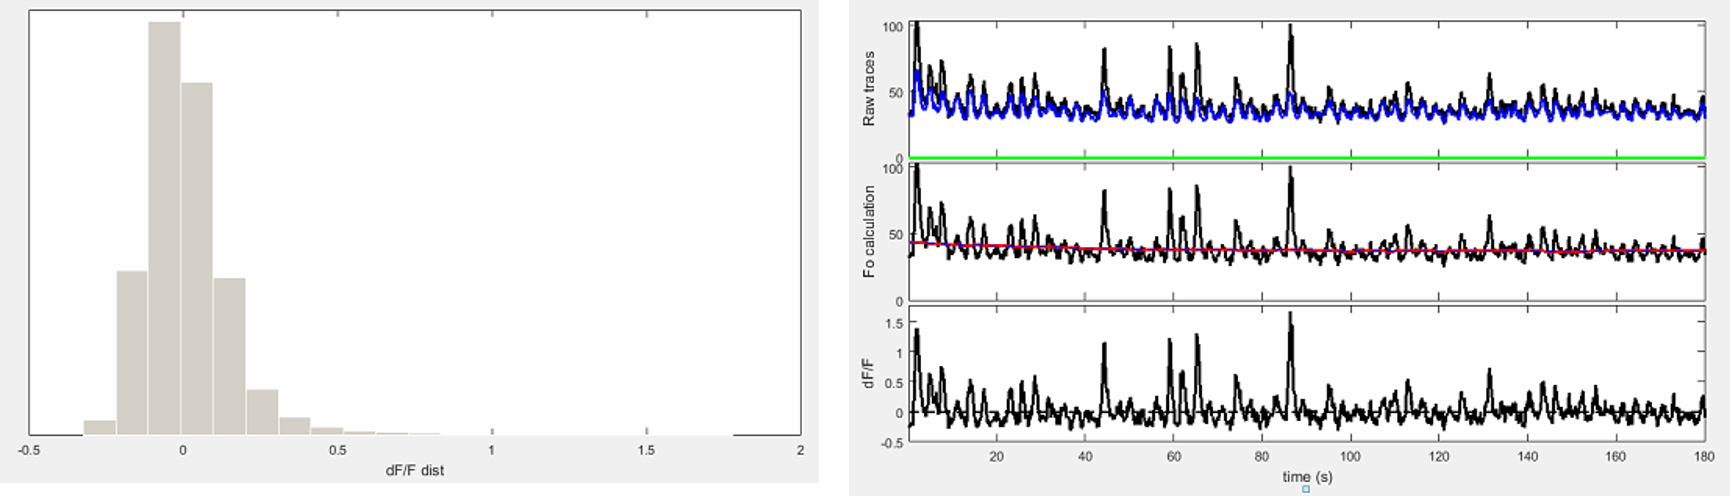
\includegraphics[width=15cm,height=15cm,keepaspectratio]{Figures/7.Results/ftraces/dFoverF.png} 
\caption{$\Delta F/F$ computation and results for an example ROI.
\newline \textbf{Left:} \textbf{Top} First 3 minutes section of raw fluorescence trace, F, for the example ROI (black trace) superimposed with the fluorescence baseline estimation trace for that ROI done by using a 60 s sliding window to discard trace's tails (blue trace); \textbf{Middle} Same fluorescence trace (black trace) superimposed with the baseline estimation value, $F_0$ (red trace), calculated as the average result of the baseline estimation trace in the top panel's blue trace, over the full session; \textbf{Bottom} $\Delta F/F$, computed as $\dfrac{F-F_0}{F_0}$.
\newline \textbf{Right:} Example ROI's $\Delta F/F$ distribution histogram. Cell's responses are mostly distributed around zero, with positive tails corresponding to spike responses.
\label{dfoverf}}
\end{figure}

Reviewing the process, we start with intrisic optical imaging on the subjects, to assess each animal's retinotopy maps and find the corresponding center field of view V1 encoding locations. 

We use two-photon imaging at that found location (with more thorough search for the center locations with the tuning protocol), and acquire brain recording sets of images of that brain's location GCaMP6s activity-related fluorescence values, for 4 different depth planes, while the subjects are shown stimuli (RF, tuning and SM protocols). 

These extracted raw images are then registered, and run through Suit2p pipeline, to select ROIs according to pixels temporal and spacial correlations in the image. These ROIs' pixels' fluorescence levels are averaged over that region and neuropil corrected. This results in raw fluorescence traces over the session's time.

With these, $\Delta F/F$ responses are computed. These are the processed data to map to the presented stimuli and use in the following analysis.

\section{RF analysis}

At each session's end, a RF analysis was held to assess whether the V1 imaged position corresponded to neurons with RFs centred in the center of the visual field, as these were the fixed intended positions for the subsequent SM spatial structure analysis.

Responses of each ROI were baseline subtracted and analysed trial by trial, mapping each trial's response to the visual field position that the corresponding stimulus was presented at (figure \ref{rfanalysis}, left panels).

Then, these responses were averaged over repetition trials, portraying mean response levels for each of the visual field positions (figure \ref{rfanalysis}, middle panels).

Finally, normalized gray-scale maps were produced for the response maps $R(az, el)$, with $az$ and $el$ the azimuth and elevation retinotopic coordinates, averaging over time on each of the positions' mean trace responses (figure \ref{rfanalysis}, right panels).

\begin{figure}[H] \centering 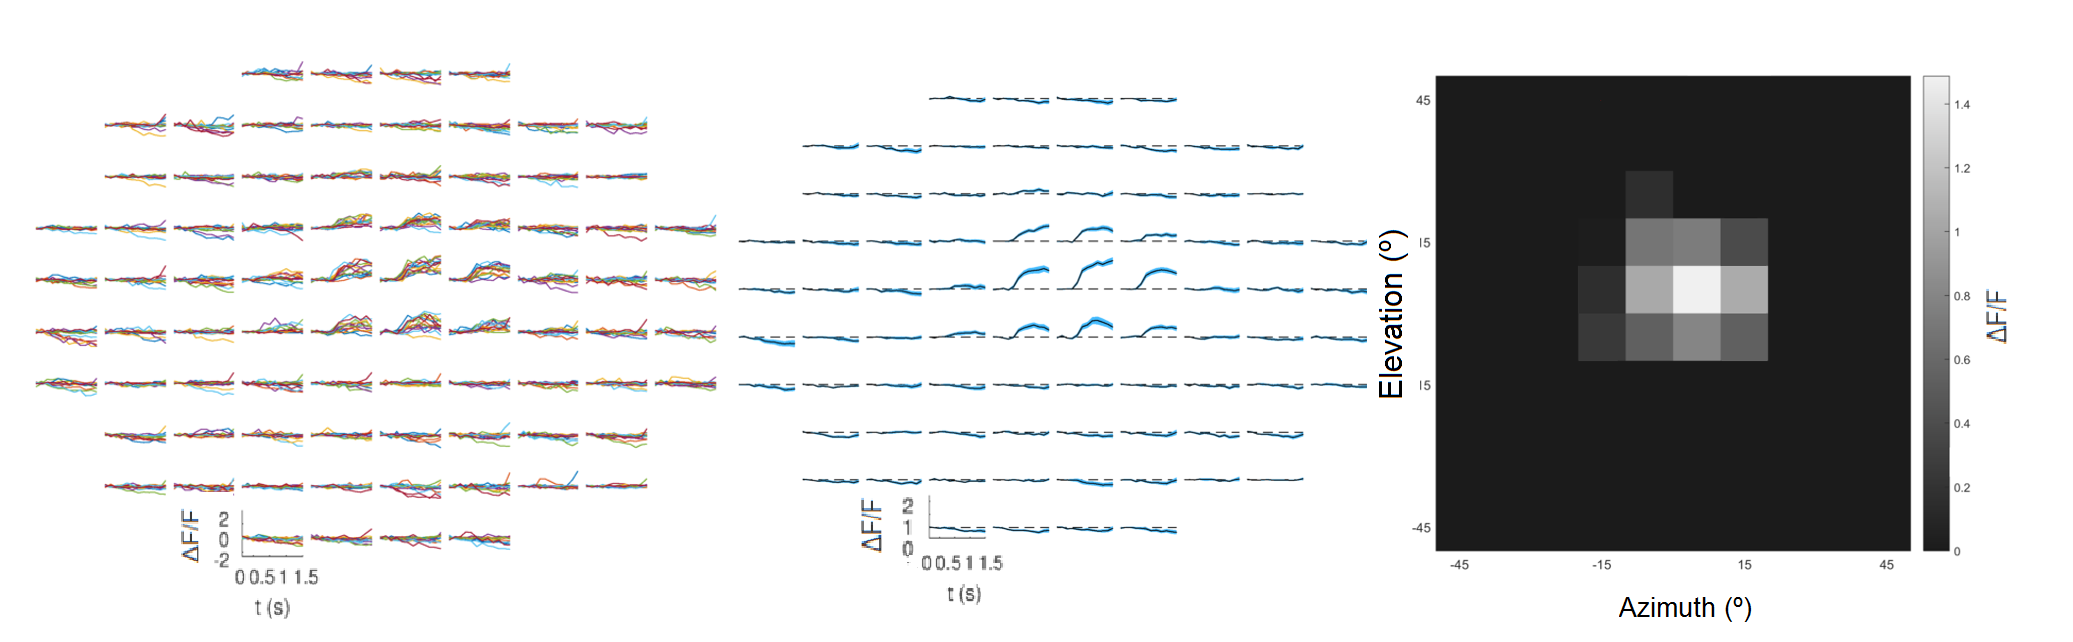
\includegraphics[width=16.2cm,height=16.2cm,keepaspectratio]{Figures/7.Results/rf/rf1.png} 
\caption{Example cell with well centred RF. 
\newline \textbf{Left:} Individual traces. Each of the 14 trial-type repetition trace response is represented in a different colour, for each of the visual field stimulated region. 
\newline \textbf{Middle:} Mean traces. Average traces over the 14 repetitions, represented also for each azimuth and elevation center stimulus condition. 
\newline \textbf{Right:}RF map. Response strengths to each of the stimulus positions, in a gray-scaled colour map.}
\label{rfanalysis}
\end{figure}

Each of these neurons' response maps was fitted to 2D-Gaussian ellipses, using Matlab implementation of the least-squares Levenberg-Marquardt algorithm (as in \cite{Marques2018}):

\begin{dmath}
R(az,el)=a+b\times \exp \left[ - \left( \dfrac{az-az_0}\times \cos(\theta)+ el-el_0)\times \sin(\theta){\sqrt{2} \times \sigma_1}\right)^2 - \left( \dfrac{-(az-az_0) \times sin \theta + (el-el_0)\times \cos(\theta)}{\sqrt{2} \times \sigma_2}\right)^2\right]
\end{dmath}

with $(az_0, el_0)$ the 2D Gaussian center coordinates, $\sigma_1$ and $\sigma_2$ the standard deviations of the gaussian across the two dimensions, $\theta$ the rotation angle between the gaussian and the $(az,el)$ axis, $a$ an offset parameter and $b$ an amplitude parameter.

The RF was then defined as the ellipse centred at $(az_0, ele_0)$ and limited by the standard deviations  ($\sigma_1$, $\sigma_2$):

\begin{equation}
\left[ \left( \dfrac{(az-az_0)\cdot \cos(\theta) + (el-el_0)\cdot \sin(\theta)}{\sigma_1}\right)^2 + \left(\dfrac{-(az-az_0)\cdot \sin(\theta) + (el-el_0)\cdot \cos(\theta)}{\sigma_2}\right)^2\right]=1
\end{equation}

The subsequent analysis was restricted to fits with $R^2>0.5$, as lower values corresponded to RF unreliable estimations. Within 10 sessions with 4 planes each, across 4 animals, 3168 out of 4198 dataset ROIs ($75\%$) were considered.

Analysing plane by plane, for each animal and session (example planes in figure \ref{ellipses}), one could assess that most of the considered RF centres were placed with similar centres within the retinotopical space, as theoretically expected for the short distances of $200 \times 200) \mu m$ imaged V1 planes. 

Two of the sessions showed very high elevation RFs, and were thus discarded for subsequent analysis, leaving 2772 measured RF cells and a total of 3728 cells ($74\%$ fitted RFs) to be analysed in regards to SM effects.

\begin{figure}[H] \centering 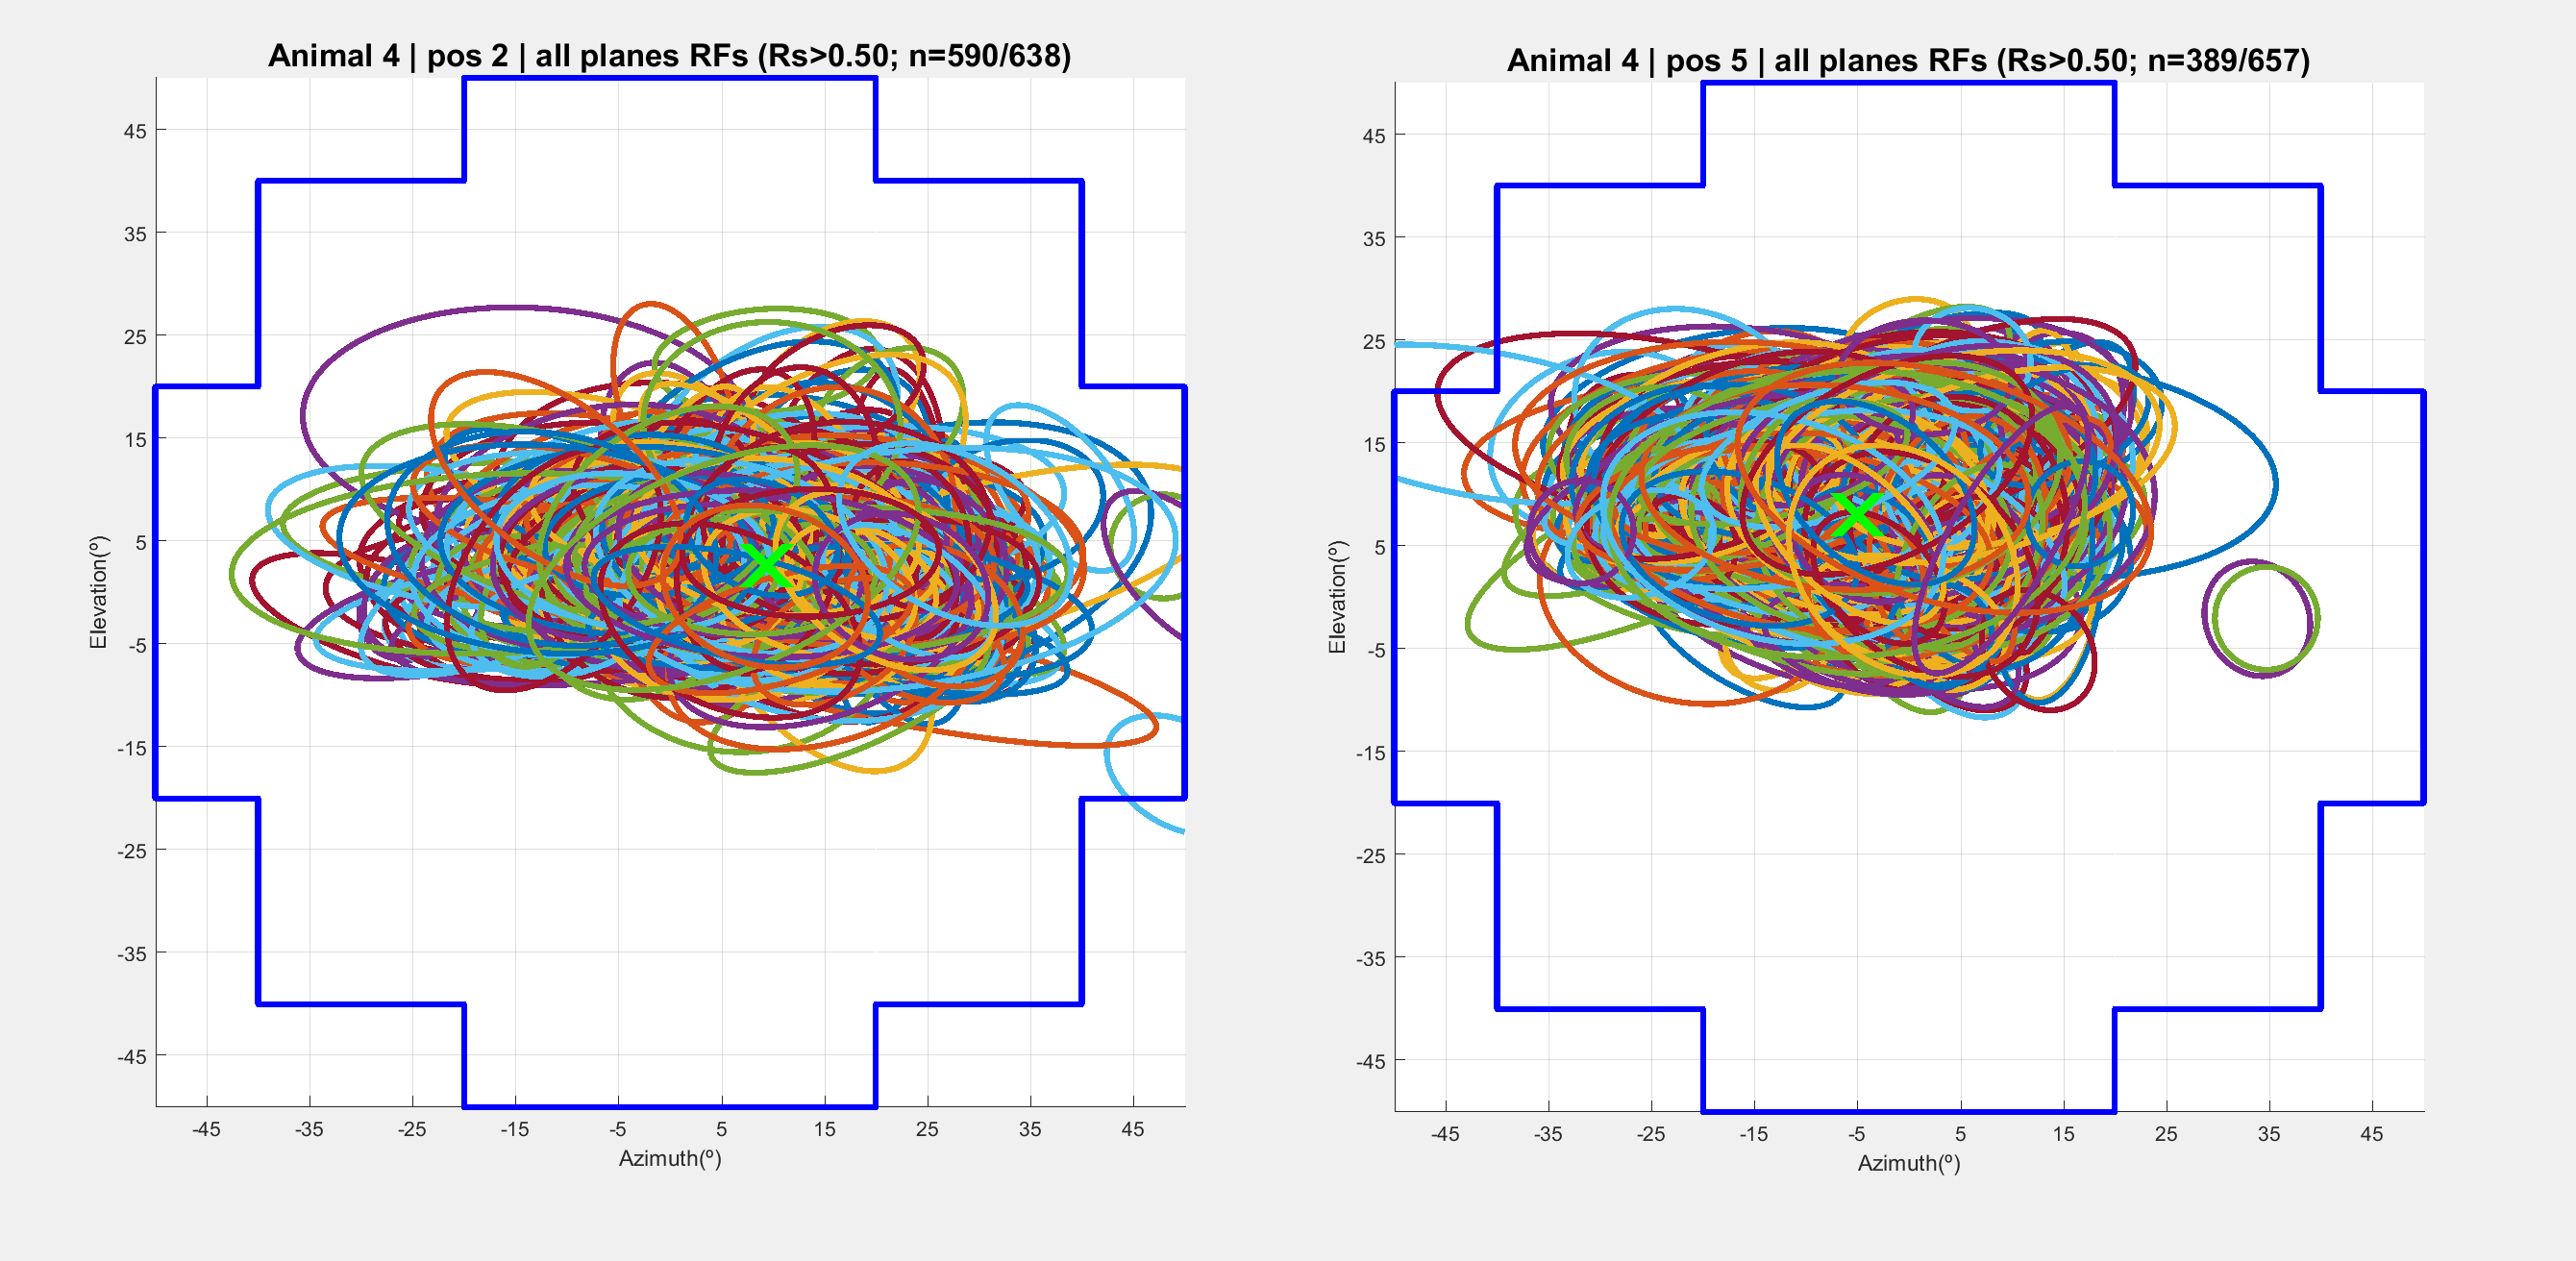
\includegraphics[width=13cm,height=13cm,keepaspectratio]{Figures/7.Results/rf/ellipsesAnimal4pos2andpos5.png} 
\caption{Superimposed 2D gaussian ellipsoidal fits for each neuron in the same plane. Two planes from two different sessions with the same animal are presented as examples.}
\label{ellipses}
\end{figure}

\section{Tuning analysis}
\label{tuningresults}

To validate bpod's tuning protocol, the selected neurons were analysed in regards to their direction (8 directions), spatial (2) and temporal (2) frequencies tuning selectivity.

Neurons in V1 can have orientation selectivity (\cite{Hubel1959}, \cite{Hubel1962}), that is, respond more strongly to a preferred orientation than to any other orientation. For mice, these orientation-selective (OS) cells are not organized into functional columns as they are for carnivores and primates (\cite{Hubel1962}), yet they do present strong orientation selectivity.

Moreover, a subset of  OS cells are also direction-selective (DS): these respond most strongly to a preferred direction than to any other.

For orientation analysis, responses of opposite directions are averaged together, and ploted on polar coordinates (figures \ref{tuninganalysisOS} and \ref{tuninganalysisDS}). The vector sum of responses at each individual trial (combining the trials for each of the same orientation opposed directions) then forms the \textit{orientation vector} of that trial. The orientation vectors for all trials then exhibit the cell's orientation tuning properties.
In the analogous way, for direction analysis, each trial measurement is binned to different direction labels, and the vector sum of the responses at individual directions then amounts to a direction vector for each trial. Direction vectors for all trials represent the cell's direction tuning properties.

Statistical significance is assessed with vector-based Hotelling's $t^2$-tests with confidence of 95\% in this project's case, to ask whether the 2D mean of the distribution of orientation and or direction vectors differ from (0,0).
 
 For any orientation, if the responses to a given orientation are significantly higher than responses to any other orientation, then the former is called the neuron's preferred orientation. This differential effect can be measured with an orientation selectivity index (OSI), for the preferred orientation response in the considered space. With  $R_{pref_or}$ the responses to the preferred orientation and $R_{orth}$ the responses to the orientation orthogonal to the preferred:
\begin{equation}
\text{OSI}= \dfrac{R_{pref \_or} - R_{orth}}{R_{pref \_or} + R_{orth}}
\end{equation}

Similarly, in the direction space, a preferred direction can also be determined for neurons that have significantly higher responses in one direction than they do in the null direction relative to the former. A DSI can be computed, for the direction doublet:

\begin{equation}
\text{DSI}=\dfrac{R_{pref} - R_{null}}{R_{pref} + R_{null}}
\end{equation}

In regards to the spatial and frequency tuning, here we used a restricted $(2 \times 2)$ space and found that for most cells, in this space, the preferred spatial frequency was of 0.04 cycles per degree and the preferred temporal frequency was at 1 Hz. These were the frequency specifications used in both the RF protocol and the SM protocol.

Here, we present two example cell responses for the different stimulus conditions in the tuning protocol: an OS cell (figure \ref{tuninganalysisOS}) and a DS cell (figure \ref{tuninganalysisDS}).

\begin{figure}[H] \centering 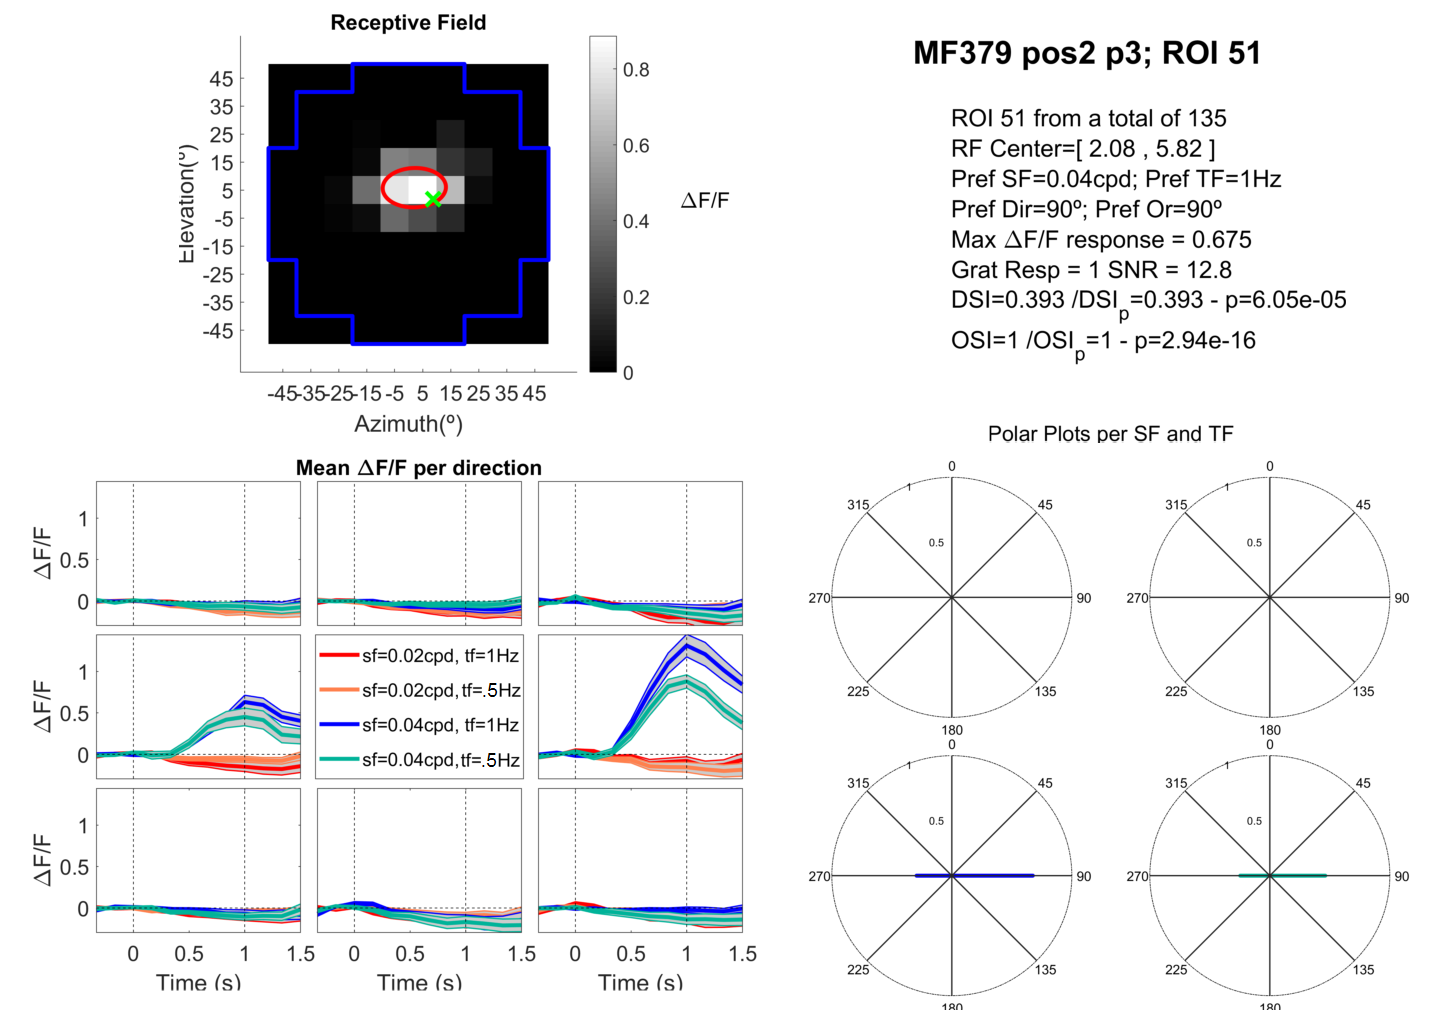
\includegraphics[width=12cm,height=12cm,keepaspectratio]{Figures/7.Results/tuning/MF379_pos2_p3_ROI0051.png} 
\caption{Tuning analysis for an example OS cell. Preferred $SF=0.04 cpd$, $TF=1 Hz$, up direction and vertical orientation. $DSI=1$ ($p=1.87 \cdot 10^{-5}$), $OSI=0.967$ ($p=3.4 \cdot 10^{-4}$).}
\label{tuninganalysisOS}
\end{figure}

\begin{figure}[H] \centering 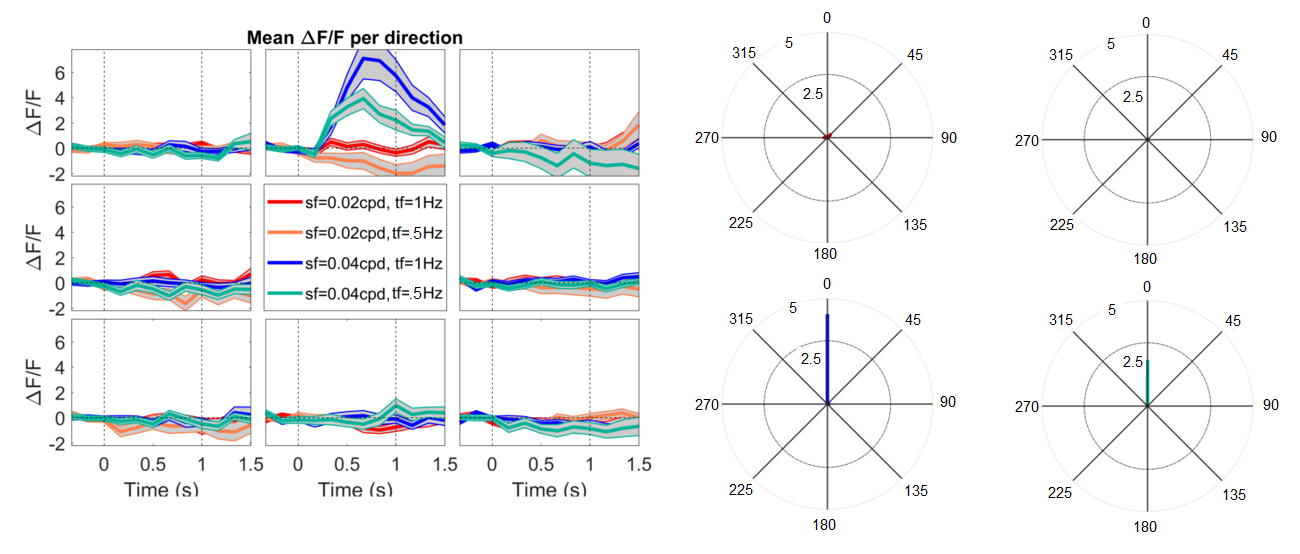
\includegraphics[width=12.5cm,height=12.5cm,keepaspectratio]{Figures/7.Results/tuning/CM006_pos1_p4_ROI0138.png} 
\caption{Tuning analysis for an example DS cell. Preferred $SF=0.04 cpd$, $TF=1 Hz$, temporal direction and horizontal orientation. DSI=0.393 ($p=6.05 \cdot 10^{-5}$), OSI=1 ($p=6.05 \cdot 10^{-5}$).}
\label{tuninganalysisDS}
\end{figure}

\subsection{Surround modulation analysis}
\label{cap:Methods}

SM analysis started with the mapping of responses during the protocol to corresponding stimuli types, from the 124 possible ones. During the experiments, 20 repetitions were held for most sessions. However, in the analysis, it was noticeable that responses decreased a lot in the second part of the protocol, possibly due to anaesthesia cumulative effects and/or adaptation to the stimuli. Therefore, to prevent from adding noise to averaged measurements, the subsequent analysis was using only the 10 first repetitions of each trial type.

Trial types were ordered in a given structure:

\begin{itemize}
\item \textbf{[1:4]} S1T, at the four directions (up, temporal, down, nasal); 
\item \textbf{[5:8]} C, analogous to above; 
\item \textbf{[9:12]} S1B, analogous to above;
\item \textbf{[13:16]} S1L, analogous to above;
\item \textbf{[17:20]} S1R, analogous to above; 
21:36 S1T+C, with first quarter (21:24) center up and surround in the 4 directions (up, temporal, down, nasal), second quarter (25:28) center temporal and surround in the 4 directions, third quarter (29:32) center down and surround in the 4 directions, and fourth quarter (33:36) center nasal and surround in the 4 directions;
\item \textbf{[37:52]} S1B+C, analogous to above;
\item \textbf{[53:68]} S1L+C, analogous to above;
\item \textbf{[69:84]} S1R+C, analogous to above;
\item \textbf{[85:100]} S2H+C, with first quarter (85:100) center up and the two horizontally positioned surrounds in the same of 4 directions (up, temporal, down, nasal), second quarter (89:92) center temporal and surrounds in the same of 4 directions, third quarter (93:96) center down and surrounds in the same of 4 directions, and fourth quarter (97:100) center nasal and surrounds in the the same of 4 directions;
\item \textbf{[101:104]} S2H, at the four directions (up, temporal, down, nasal);
\item \textbf{[105:120]} S2V+C, with first quarter (105:108) center up and the two vertically positioned surrounds in the same of 4 directions (up, temporal, down, nasal), second quarter (109:112) center temporal and surrounds in the same of 4 directions, third quarter (113:116) center down and surrounds in the same of 4 directions, and fourth quarter (117:120) center nasal and surrounds in the the same of 4 directions;
\item \textbf{[121:124]} S2V, at the four directions (up, temporal, down, nasal);
\end{itemize}